%%%%%%%%%%%%%%%%%%%%%%%%%%%%%%%%%%%%%%%%%
% Arsclassica Article
% LaTeX Template
% Version 1.1 (10/6/14)
%
% This template has been downloaded from:
% http://www.LaTeXTemplates.com
%
% Original author:
% Lorenzo Pantieri (http://www.lorenzopantieri.net) with extensive modifications by:
% Vel (vel@latextemplates.com)
%
% License:
% CC BY-NC-SA 3.0 (http://creativecommons.org/licenses/by-nc-sa/3.0/)
%
%%%%%%%%%%%%%%%%%%%%%%%%%%%%%%%%%%%%%%%%%

%----------------------------------------------------------------------------------------
%	PACKAGES AND OTHER DOCUMENT CONFIGURATIONS
%----------------------------------------------------------------------------------------

\documentclass[
10pt, % Main document font size
letterpaper, % Paper type, use 'letterpaper' for US Letter paper
oneside, % One page layout (no page indentation)
%twoside, % Two page layout (page indentation for binding and different headers)
headinclude,footinclude, % Extra spacing for the header and footer
english
]{article}

%%%%%%%%%%%%%%%%%%%%%%%%%%%%%%%%%%%%%%%%%
% Arsclassica Article
% Structure Specification File
%
% This file has been downloaded from:
% http://www.LaTeXTemplates.com
%
% Original author:
% Lorenzo Pantieri (http://www.lorenzopantieri.net) with extensive modifications by:
% Vel (vel@latextemplates.com)
%
% License:
% CC BY-NC-SA 3.0 (http://creativecommons.org/licenses/by-nc-sa/3.0/)
%
%%%%%%%%%%%%%%%%%%%%%%%%%%%%%%%%%%%%%%%%%

%----------------------------------------------------------------------------------------
%	REQUIRED PACKAGES
%----------------------------------------------------------------------------------------

\usepackage[
nochapters, % Turn off chapters since this is an article        
beramono, % Use the Bera Mono font for monospaced text (\texttt)
eulermath,% Use the Euler font for mathematics
pdfspacing, % Makes use of pdftex’ letter spacing capabilities via the microtype package
dottedtoc % Dotted lines leading to the page numbers in the table of contents
]{classicthesis} % The layout is based on the Classic Thesis style

\usepackage{arsclassica} % Modifies the Classic Thesis package

\usepackage[T1]{fontenc} % Use 8-bit encoding that has 256 glyphs

\usepackage[utf8]{inputenc} % Required for including letters with accents

\usepackage{graphicx} % Required for including images
\graphicspath{{Figures/}} % Set the default folder for images

\usepackage{enumitem} % Required for manipulating the whitespace between and within lists

\usepackage{lipsum} % Used for inserting dummy 'Lorem ipsum' text into the template

\usepackage{subfig} % Required for creating figures with multiple parts (subfigures)

\usepackage{amsmath,amssymb,amsthm} % For including math equations, theorems, symbols, etc

\usepackage{varioref} % More descriptive referencing

%----------------------------------------------------------------------------------------
%	THEOREM STYLES
%---------------------------------------------------------------------------------------

\theoremstyle{definition} % Define theorem styles here based on the definition style (used for definitions and examples)
\newtheorem{definition}{Definition}

\theoremstyle{plain} % Define theorem styles here based on the plain style (used for theorems, lemmas, propositions)
\newtheorem{theorem}{Theorem}

\theoremstyle{remark} % Define theorem styles here based on the remark style (used for remarks and notes)

%----------------------------------------------------------------------------------------
%	HYPERLINKS
%---------------------------------------------------------------------------------------

\hypersetup{
%draft, % Uncomment to remove all links (useful for printing in black and white)
colorlinks=true, breaklinks=true, bookmarks=true,bookmarksnumbered,
urlcolor=webbrown, linkcolor=RoyalBlue, citecolor=webgreen, % Link colors
pdftitle={}, % PDF title
pdfauthor={\textcopyright}, % PDF Author
pdfsubject={}, % PDF Subject
pdfkeywords={}, % PDF Keywords
pdfcreator={pdfLaTeX}, % PDF Creator
pdfproducer={LaTeX with hyperref and ClassicThesis} % PDF producer
} % Include the structure.tex file which specified the document structure and layout
\usepackage[letterpaper]{geometry}
\geometry{verbose,tmargin=1in,bmargin=1.3in,lmargin=1.45in,rmargin=1.45in}

\hyphenation{Fortran hy-phen-ation} % Specify custom hyphenation points in words with dashes where you would like hyphenation to occur, or alternatively, don't put any dashes in a word to stop hyphenation altogether

%----------------------------------------------------------------------------------------
%	TITLE AND AUTHOR(S)
%----------------------------------------------------------------------------------------

\title{\normalfont\spacedallcaps{CIS 559 Project 3:\break Gunslinger}} % The article title

\author{\spacedlowsmallcaps{Ian Sibner, David Liao, Nikhil Roy}} % The article author(s) - author affiliations need to be specified in the AUTHOR AFFILIATIONS block

\date{20 October 2015} % An optional date to appear under the author(s)

%----------------------------------------------------------------------------------------
\setlength\parindent{0pt}
\setlength{\parskip}{1em}

\usepackage[section]{placeins}

\begin{document}

%----------------------------------------------------------------------------------------
%	HEADERS
%----------------------------------------------------------------------------------------

\renewcommand{\sectionmark}[1]{\markright{\spacedlowsmallcaps{#1}}} % The header for all pages (oneside) or for even pages (twoside)
%\renewcommand{\subsectionmark}[1]{\markright{\thesubsection~#1}} % Uncomment when using the twoside option - this modifies the header on odd pages
\lehead{\mbox{\llap{\small\thepage\kern1em\color{halfgray} \vline}\color{halfgray}\hspace{0.5em}\rightmark\hfil}} % The header style

\pagestyle{scrheadings} % Enable the headers specified in this block

%----------------------------------------------------------------------------------------
%	TABLE OF CONTENTS & LISTS OF FIGURES AND TABLES
%----------------------------------------------------------------------------------------

\maketitle % Print the title/author/date block

\setcounter{tocdepth}{2} % Set the depth of the table of contents to show sections and subsections only

\tableofcontents % Print the table of contents

\listoffigures % Print the list of figures

% \listoftables % Print the list of tables

%----------------------------------------------------------------------------------------
%	ABSTRACT
%----------------------------------------------------------------------------------------

\section{Introduction} % This section will not appear in the table of contents due to the star (\section*)

Gunslinger is an $n$-player game where each player is initialize with two disjoint sets of $f$ friendly players (\textit{friends}) and $e$ enemy players (\textit{enemies}). This implies that $e + f < n$ since the player will not have itself as a friend or enemy. The friend relationship is symmetric, so if A is a friend of B, then B is a friend of A; the enemy relationship, however, may be asymmetric.

Each turn, each player can fire one shot in an attempt to kill another player. However, a player is not killed unless two players shoot it simultaneously. Once dead, a player can no longer shoot. The game ends when the set of living players remains unchanged for 10 rounds in a row, whether or not players are still shooting. Each players' objective is have the highest number of points at the end of the round. Points are awarded as follows:
\begin{enumerate}
  \item One point for surviving until the end of the round.
  \item One point for each surviving friend (maximum $f$).
  \item One point for each dead enemy (maximum $e$).
\end{enumerate}

Players retain perfect information about who shot whom in previous rounds.

\section{Initial Insights and Observations}

Immediately, our team observed several key features about the game.

\begin{enumerate}
  \item While players are given a list of allies and enemies, there are more opponents than just those given. Players who we perceive neutrally could target us as an enemy. This lead us to believe that we might consider targeting those players as well to preserve our wellbeing.
  \item A way to model the state of the game as perceived by our player would be to create a dynamic enmity graph. This would help us keep track of the relationships between all players
  \item We needed to consider whether or not an aggressive or non-aggressive approach would be better. As a proactive player, targeting our enemies might lead others to target us (if we target their allies and they choose to defend them). On the other hand, taking a retaliatory approach might limit our influence on the game end state.
  \item Winning the game meant having the highest score. By killing off other players, we would be able to raise our own rank by lowering other players' score.
\end{enumerate}

These insights guided our strategy throughout and allowed us to focus on the most important aspects of the game.

\section{Strategies and Concepts}

\subsection{David's Revenge}

David's Revenge was our initial attempt where we tried to create a retaliatory player. The main idea was to maintain our own player's wellbeing while minimizing involvement if at all possible. The only times that David's Revenge would take action is if an arbitrary player targeted our player.

We initially construct an enmity graph. An enmity graph captures which players seem to be enemies of others. This provided us with more than enough information to design our player's decision making. We only consider any player that targeted us.

Using our enmity graph, we identify players that have targeted us and choose a player to return fire. The choice in player evolved through many designs. Initially it was the most recent player that shot us, but later on it became a weighted selection based on the number of times the player targeted us. We used a bounding ``window'' to make more recent hits more relevant as opposed to more temporally distant hits.

If a player stopped targeting us, as long as they are within our defined time window, we would still target them. If we had no player target us at all in the first place, we would simply take no action.

\subsection{EV Player}
The general strategy of EV player was made up of two phases. The first phase involved creating a directed graph where each edge represents the probability of one player shooting another on the next turn. The second phase dealt with using these probabilities to accurately compute the expected value of points gained from shooting each player and not shooting at all. Ultimately, this player would shoot whichever option yielded the highest number of expected points. 

Graph Creation:

In order to predict probabilities of one player shooting another we clearly need to refer to the past shooting events. Whenever a player shoots another, it contributes to his probability of shooting that player in the future (assuming his target is still alive in the future). The more recent the shot has occurs, the more likely it is that the same shot will occur again on the next turn. 


EV Calculation:

Now that we have approximations for the probability that any player shoots another player, we can apply these probabilities to come up with expected points to be gained or lost by making a certain decision. When shooting a player, there are three ways your expected point total can be affected: 

1) Expected enemies killed can increase

2) Expected friends that remain can increase

3) Expectation for surviving till the end can decrease

Note that these expectations are calculated relative to the option of not shooting, so if we see negative expectations for shooting all of the players, the player will simply not shoot.


\subsection{David's Revenge's Revenge}

As the name suggests, David's Revenge's Revenge (DRR for short) was built directly on top of David's Revenge. Determining who to shoot is the exact same as David's Revenge: when DRR shoots, it will shoot the enemy who shot it most in previous rounds. However, unlike David's Revenge, DRR does not shoot whenever it can. It uses a logistic function in order to determine a \textit{shooting percentage}, and then shoots with a probability equal to this function value.

The intuition behind the logistic function is that in situations with lots of friends, it is better to be conservative with shooting. The friends of the enemy you shot are likely to retaliate in subsequent rounds, so a player that is too aggressive in these situations is likely to die. However, in situations with few friends, being aggressive makes more sense because retaliation is unlikely. This applies regardless of the number of actual enemies; it generally pays off to target neutral players as well, as long as there are few friends, because it improves a players' \textit{relative} ranking compared to other players. It was noted by Spriha that this might bring down a players' ranking in certain situations because it would eliminate another player's enemy; however, as we will see in the results section, we actually did quite well in situations where there were many enemies.

Thus we used the ratio of non-friends to players as the independent variable in the logistic function: $x = \dfrac{n - f}{n}$. Then the shooting percentage is calculated as $P = \dfrac{1}{1 + e^{-\frac{x - \mu}{\beta}}}$, where $\beta$ and $\mu$ govern the steepness and the mean of the distribution respectively. Initially, our logistic curve had $\beta=0.07,\mu=0.07$ (see Figure 1). However, we wanted to find the best-performing combination, so we systematically tried different combinations of $\mu$ and $\beta$ to find out which produced the best rank. In the end, we found that $\beta=0.06,\mu=0.4$ (see figure 2) was the best performing. This curve was more aggressive than the original curve; it appears that shooting more often improves performance even at relatively low non-friend to players ratio, reaching 90\% at an x-value of just 60\%.

\begin{figure}[h]
\centering
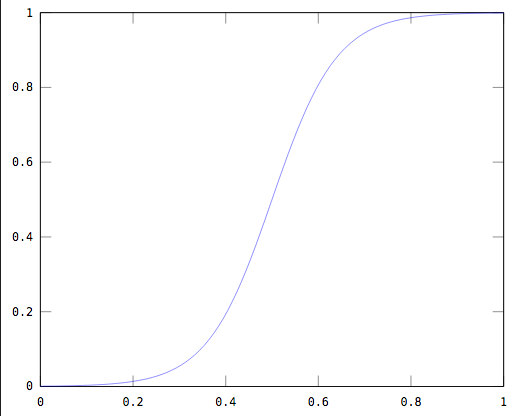
\includegraphics[width=0.8\columnwidth]{old-logistic-curve.png}
\caption[Initial logistic curve with $\beta=0.07,\mu=0.5$]{Initial Logistic Curve with $\beta=0.07,\mu=0.5$}
\label{fig:gallery2}
\end{figure}

\begin{figure}[h]
\centering
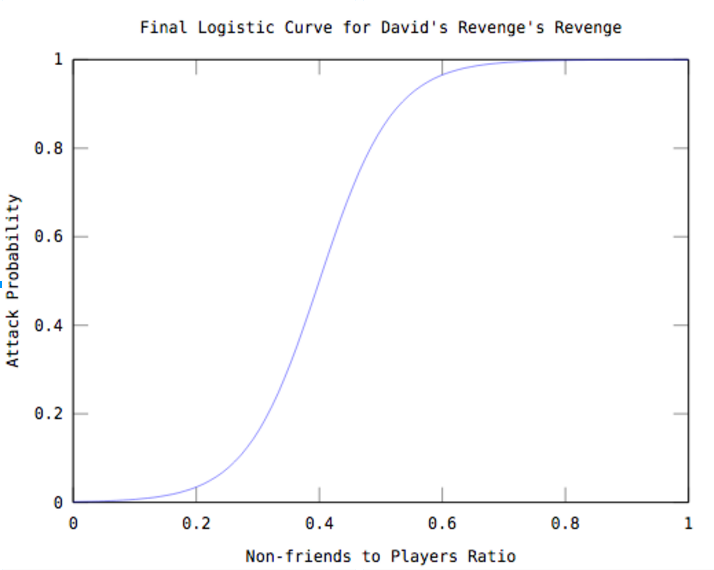
\includegraphics[width=0.8\columnwidth]{new-logistic-curve.png}
\caption[Final logistic curve with $\beta=0.06,\mu=0.4$]{Final logistic curve with $\beta=0.06,\mu=0.4$}
\label{fig:gallery3}
\end{figure}
\section{Implementation}

\subsection{David's Revenge}

David's Revenge took a very simplistic approach in defining its actions. In its final iteration, it featured a selection of a target (if one existed) based on the most hits against us in a time window. Formally, in a game of $n$ players let $p_{it}$ be the player in position $1\le i<n$ clockwise from our player at round $t$. $p_{it} \in {0,1}$ where it is $0$ if it does not hit us and $1$ if it does. Then at round $t'$, our player will target $argmax_i$ $\{P_i | P_i = \sum_{t'-k}^{t'}p_{it}\}$. Our look-back window in this case is $k$.

To compute this, we cache all hits from the start of the game by leveraging our enmity graph. We iterate through the past $k$ rounds and count up how many times each player hit us throughout those $k$ rounds. We then select the player with the largest sum and choose to hit that person. Thus if no player targeted us in a round, however within the past few rounds there had been players that targeted us, we would look to target those players.


\subsection{EV Player}


Graph Creation:
\\
A shooting history is maintained that keeps track of every player’s moves. The specific history for a player is an ordered list containing either the player id of player that was shot on that specific round or a -1 indicating that no one was shot. The player model’s the probability of one player shooting another by using the geometric series. The most recent shot receives a weighting of 1/2, the next most recent receives a weighting of 1/4, the one after that receives 1/8 and so on and so forth. After this process, the probabilities are added up for each unique player. Note that shot history includes a “blank” or the event in which no shot is taken. The act of not shooting is essentially treated as a separate player in this sense and is assigned a probability just like the other players are. One more subtlety to note is that once player’s get eliminated there is a probability of 0 that they will be shot. The way we reflect this result in our algorithm is by removing all dead players from every shot history list on every turn.  Below we have included a sample sequence for one player's shooting history. 
\\
\\


\begin{figure}[h]
\centering
\includegraphics[width=0.5\columnwidth]{geometric_final.png}
\caption[Final logistic curve with $\beta=0.06,\mu=0.4$]{Sample 3 step sequence}
\label{fig:gallery3}
\end{figure}


EV calculation: 

As mentioned before, there are three different aspects that contribute to a player’s total expected points. EV player carries out the following calculations to produce expected values:
\\
\\
\\
Expected enemies killed: 

For this value, we are not simply looking to determine the probability that some enemy player p will be shot at. We want to compare the probability that p will be shot at at least once next turn to the probability that p will be dead next turn (have two or more players shoot at it). Obviously, if both of these values are similar, there is no need to shoot. Our expected value is essentially the value gained by shooting. Thus, this can be computed using the following formula: 

E(enemies killed) = P(p is shot at least once) - P(p is shot at least twice) 
\\
\\
\\
Expected friends saved:

This value is slightly more complicated to calculate. Ultimately, our expected value should be the probability that the player p that we are targeting will shoot a friend of our’s multiplied by the probability that this friend will receive at least one other shot from someone else. If this friend has a very small chance of getting shot at by anywhere else besides the one player we are targeting, it makes no sense to defend our friend. From this value we will subtract the probability that this friend of ours will die next turn (if we don’t shoot at him). If our friend is extremely likely to die, there’s no sense in wasting a bullet trying to save him/her. We compute this value using the following formula:

E(friends saved) = (P(f is shot at least twice | p is alive) - P(f is shot at least twice | p is dead) ) * P(p is shot at least once)
\\
\\
\\

Expectation of survival:

Every time our player chooses to shoot, it loses value because it’s probability of dying (and losing a point as a result) increases. This value depends on the ratio of enemies to total players. In a game where there are mostly friends and very few enemies, a high percentage of the N initial players tend to make it to the end. In games where there are many enemies, it is unlikely that more than a couple of players will be remaining. As a result, EV player roughly models this probability as $0.7 * (e/N)$.

Note that calculating some of the probabilities above using our probability graph is not trivial. P(p is shot at least once) can be obtained by subtracting the product of the probabilities that every player does not shoot p from 1. Similarly, P(p is shot at least twice) would involve subtracting the total probability that p is shot at exactly 0 or 1 times from 1. 
\subsection{David's Revenge's Revenge}

The implementation of David's Revenge's Revenge was straightforward, given the existing code for David's Revenge. We implemented the logistic curve in another class, which was parametrized by the values of $\mu$ and $\beta$. Once we had the final values of $\mu$ and $\beta$ then we simply hardcoded them in the David's Revenge's Revenge constructor, and added a check to the end comparing \texttt{Math.random()} to the value from the Logistic Curve to implement the probability calculation.

The more interesting part of the implementation of DRR was \textit{determining} the best values of $\mu$ and $\beta$. To do this, we first modified the player to take in parameters from a file so that it would be easier to automate changing the variables. We also modified the tournament code so that it would only print out the average ranking (which was the metric we were using to measure performance). Then we wrote two JavaScript programs: the first collected all the results for all the parameter combinations, and the second parsed the text results to determine the best-performing combination.

\section{Results}
Our results were mixed in the end-of-class tournaments. In the free-for-all tournaments, we came within the top 3 (by average rank) in the following configurations:
\begin{itemize}
  \item 6 enemies, 0 friends
  \item 6 enemies, 1 friend
  \item 17 enemies, 0 friends
\end{itemize}

In other configurations, we generally came in somewhere in the middle; however, this is not very impressive considering that the dumbest players (including the totally-random ``dumb player'') were active in this tournament.

In the best-player tournaments, we came within the top 2 (by average rank) in these configurations:
\begin{itemize}
  \item 1 enemy, 0 friends
  \item 2 enemies, 0 friends
  \item 2 enemies, 1 friend
\end{itemize}

There were some configurations in which we did relatively poorly, however. Here are those in which we came in last:
\begin{itemize}
  \item 5 enemies, 0 friends
  \item 4 enemies, 1 friend
  \item 4 enemies, 0 friends
  \item 3 enemies, 0 friends
  \item 0 enemies, 2 friends
\end{itemize}

There are some interesting patterns here. In free-for-all play, we do best in situations where we have no friends (kind of like real life). This makes sense because we don't take advantage of friends very well; we don't have any code for defending them. Furthermore, having more friends makes our player less agressive, and because of the randomness of a free-for-all this can often result in dying too early.

The best-of play is also interesting. We seem to do best in situations with \textit{more neutral players and now friends}, and poorly in situations where we have a lot of enemies or no enemies. Observing a few games, it appears that our strategy of being aggressive in situations with lots of neutral players was quite helpful: it's pretty safe to aggressively target neutral players if they don't have friends. Situations in which targeting neutal players hurts our rank (as Spriha suggested might happen) seem to be fairly rare in these configurations, given that our player was fairly successful.

In the configurations that we did poorly in, we generally had a lot of enemies and few friends. This was somewhat surprising, because we thought that our aggressive strategy in these situations would help us get some kills before being killed ourselves. However, this does make sense when we consider that many of our enemies would target players that shot them if they survived. Even if they had other enemies, they would attack us in \textit{retalation}, which meant that we would die earlier and therefore have a lower score. Perhaps if we had had time to take enemies and neutral players into account separately, we could have done better in these situations. Nevertheless, it's worth noting that the average ranks in many of these mostly-enemy configurations are within a very small range for all teams (~0.2), implying that our performance was not actually as far below the other teams as the last-place finish implies.

\section{Contributions}

We had two main contributions to the class strategy and discussion:
\begin{enumerate}
  \item \textbf{Expected value and probabilistic play -} Nikhil was the first to try and explore the value of probabilistic play, first with the strategy of Bayesian updating and then with his geometric distribution-based Expected Value Player.
  \item \textbf{Logistic curve -} Ian was the first to have the idea of using a mathematical function to vary the aggression of a player (their likelihood of shooting). This was a novel idea and lead to some good class discussions on the use of other parameters for improving this function.
\end{enumerate}

\section{Future Directions and Limitations}

\subsection{Faster Initial Spread}

Our players tended to do best on larger boards because of its high energy density. It tended not to overextend, unlike some other organisms which would tend to start dying frequently due to very aggressive population growth. But on small maps, this aggressive overextension was actually beneficial to these organisms, because they could ``choke out'' less aggressive competitors and dominate all food resources. Once their opponents went extinct, their organisms would settle into a steady state of lower population and energy compared to their initial population explosion. However, by that time, it was too late for slower-growing competitors like SimplePlayer.

Although an organism might not know the size of the board it starts on, we believe that our SimplePlayer could benefit from employing a more aggressive strategy \textit{only during the first part of the game}. The ideal length of this ``aggressive period'' might vary based on known map conditions, but based on our observations of population explosions in configurations where the total grid size was less than 1000, we believe that around 100 turns of aggressive expansion is usually sufficient to gain dominance over a large portion of the map. Once this period is up, we would switch to our current, more conservative strategy to take advantage of its natural tendency towards higher energy density. This would make our SimplePlayer much harder to choke out at the beginning, but would still allow it to take advantage of its effective conservative strategy after the intial territory grab. Following the initial population explosion, organisms that maintained aggression would tend to move more and use more energy, which would allow our less aggressive organisms to slowly chip away at their territory while maintaining a high average energy level.

\section{Acknowledgments}

The idea of an enmity graph is attributed to Group 4 who initially coined the term. Our first implementation leveraged their graph code that was already written and we extended their ideas. We would also like to thank Group 3 for hinting us that using a time window (like short-term memory) might be worth a look.

\section{Conclusion}

Overall we were pleased with the way this project went. The idea was certainly an interesting one and there was a large variety of approaches that could have been taken. Generally speaking, there are two ways to tackle this problem, deterministically or probabilistically, and we were able to pursue solutions using both approaches. The deterministic approach ended up working out better for us since the probabilistic approach may have had too many assumptions associated with it. We realized that there really isn't one optimal solution to this problem because a team's performance largely depends on the strategies being employed by other teams. Ultimately, we had a great time working on this project and achieved the goals that we had initially set. 
\end{document}
